%----------------------------------------------------------------------------
\section{Digitális Technika}
{\footnotesize Logikai függvények kapcsolástechnikai megvalósítása. Digitális áramköri családok jellemzői (TTL, CMOS, NMOS). Különböző áramköri családok csatlakoztatása. Kombinációs és szekvenciális hálózatok. A/D és D/A átalakítók.}
%----------------------------------------------------------------------------
\subsection{Logikai függvények kapcsolástechnikai megvalósítása.}
Egy-egy alapáramkör megvalósítására több áramkörtechnikai megoldás született, ezek a teljesítményfelvételben, tápfeszültségigényben, H (high) és L (low) szint feszültségben, sebességben és a kimeneti terhelhetőségben térnek el egymástól. Az áramkörcsaládok helyes megválasztásához ismernünk kell a belső felépítésüket és a bemeneti-kimeneti terhelhetőségüket is. Egy logikai kapu minden bemeneti állapotához meghatározott kimeneti állapot tartozik. A logikai kapu által megvalósított függvény nem egyértelmű, ha a szintállapot és a logikai állapot közötti kapcsolat nincs tisztázva. Ez az összerendelés lehet: pozitív logika (H=1,L=0) és lehet negatív logika (H=0,L=1) ,attól függően, hogy azt az áramkörcsaládot használjuk, amelyikkel egyszerűbb a kapcsolás. Ha negatív logikára térünk át a függvényeket a következőképpen kel megcserélnünk:\\
Nem-vagy $\leftrightarrow$ Nem-és , vagy $\leftrightarrow$ és , nem $\leftrightarrow$ nem\\ 
A fizikai megvalósításukhoz: kapcsolókat,komparátorokat,tranzisztorokat használunk. A gyakorlatban szinte minden logikai kaput Nem-és kapukkal realizálnak, olcsósága miatt.

\subsection{Digitális áramköri családok jellemzői(TTL, CMOS, NMOS).}
\subsubsection{TTL --- Tranzisztor-tranzisztor logika}
Legnagyobb típus-választékú, univerzális célra készülő bipoláris integrált áramkör rendszer. A bemenetet egy többemitteres tranzisztor szolgáltatja. Kis sebességű, így nagyobb a késleltetés az egyes kapuknál. A fogyasztása a többi családhoz képest elég nagy, de az órajel emelkedésével csak kis mértékben emelkedik és az elektromos kisülések ellen is kellően védett. 

Kis és közepes bonyolultságú integrált áramkörökben a legelterjedtebb bipoláris áramkör. A logikai áramkörökben a kapcsolási és terjedési-késleltetési idők szabják meg a sebességet, a kapunkénti disszipált teljesítmény (fogyasztás) is fontos korlátot szab a rendszernek.
Típusai:
\begin{itemize}[nosep]
	\item H (high speed)
	\item S (schottky-diódás)
	\item L (low power)
	\item LS (low power schottky)
\end{itemize}
\begin{tabular}{|c|c|c|}
	\hline 
	TTL család & Egy kapura eső fogyasztás (mW) & Terjedési-késleltetési idő (ns) \\ 
	\hline 
	normál & 20 & 10 \\ 
	\hline 
	H TTL & 30 & 6 \\ 
	\hline 
	S TTL & 20 & 3 \\ 
	\hline 
	L TTL & 2 & 35 \\ 
	\hline 
	LS TTL & 2 & 15 \\ 
	\hline 
\end{tabular} 
\paragraph{TTL nem-és kapu felépítése és működése:}~\\
U\textsubscript{t} = +5V, L szint: 0V -- 0,8V, H szint: 2,4V -- 5V\\
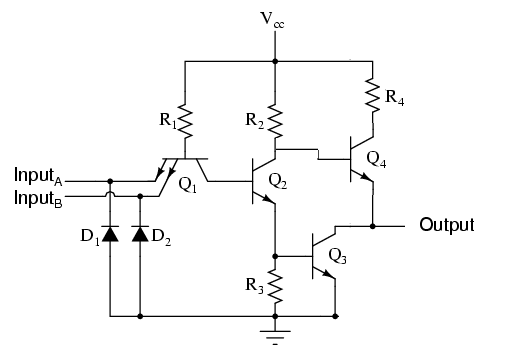
\includegraphics[width=0.5\linewidth]{fig/11-TTL_NAND_schema}
Ha a Q\textsubscript{1} tranzisztor bármelyík emitter kivezetésére 0 logikai szint kerül, a kimeneten 1-es logikai szint lesz a Q\textsubscript{4} tranzisztor és az R\textsubscript{2} ellenállás miatt. Ha a Q\textsubscript{1} tranzisztor mindkét emitter kivezetésére 1 logikai szint kerül, akkor a Q\textsubscript{2} tranzisztor kinyit, a a Q\textsubscript{4} tranzisztor lezár és a Q\textsubscript{3} tranzisztor nyitott állapota miatt alacsony logikai szintre kerül a kimenet.

\subsubsection{MOS --- Metal-Oxid-Semiconductor}
A MOS áramkörök bemenetei érzékenyek a túlfeszültséggel szemben, a megengedettnél nagyobb GATE feszültség miatt átüthet a GATE alatti vékony oxidréteg. Ennél a családnál is tranzisztorokat használnak, de a bipoláris tranzisztorok helyett a fémoxid-félvezetőből készült térvezérlésű FET, vagyis Field-effect tranzisztorokat. Ezáltal sokkal nagyobb műveleti sebességet tudnak elérni.

\subsubsection{N-MOS --- N csatornás MOS (térvezérlésű) tranzisztor}
Csak N-csatornás MOSFET-eket használ, ezáltal csak a magas jelszintet tudja stabilan megjeleníteni. Kisebb a zavarvédettsége és nagyobb a fogyasztása, de a TTL családhoz képest hasonló a CMOS családhoz, csak egyszerűbb kialakítású, ezért olcsóbb is.

Felületigénye jóval kisebb, mint a TTL-nek, gyártási technológiája is gyorsabb (kevesebb művelet), jelentősen kisebb a teljesítményfelvétele. Az N-csatornás tranzisztorok működésében részt vevő Negatív töltéshordozók mozgékonysága majdnem 3-szor nagyobb,mint a (régi technikája miatt kiszorított) P-csatornás tranzisztorok Pozitív töltéshordozóinak mozgékonysága, ezért az N-MOS áramkörök kisebb Gate-kapacitása miatt nagyobb sebességre képesek, csökken a tranzisztor U TO küszöbfeszültsége is, amely alacsonyabb tápfeszültség alkalmazását teszi lehetővé,emiatt könnyebb az N-MOS tranzisztorokat könnyű illeszteni a TTL áramkörökhöz.

\paragraph{N-MOS nem-és kapu felépítése és működése:}~\\
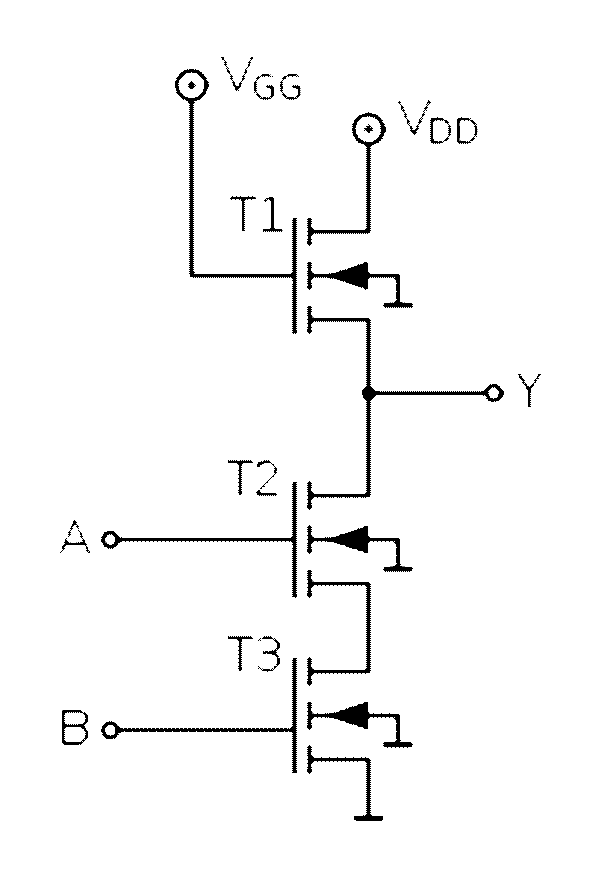
\includegraphics[width=0.5\linewidth]{fig/11-NMOS_NAND_schema1}\\
A T\textsubscript{1} tranzisztort R\textsubscript{D} (100K\textOmega) ellenállás helyett alkalmazzák a térkihasználás és a nagyobb drain ellenállás miatt. Az Y kimeneten csak akkor jelenik meg alacsony logikai színt, ha a T\textsubscript{2} és T\textsubscript{3} tranzisztor is vezet, azaz A-ra és B-re is logikai magas szintet rakunk.

A MOS kapu egyenáramú bemeneti ellenállása nagyon nagy értékű. A bemeneti feszültség változása a gate-kapacitást töltő és kisütő áramot hoz létre. Ez a rövid idejű áramimpulzus nagyobb, mint a szivárgási áram. Ennek ellenére úgy lehet venni, hogy a MOS tranzisztor nem terheli le az előző kapu kimenetét. N-MOS-ok terjedési-késleltetési ideje 15 ns körüli, a teljesítményfelvételük pár szár \textmu W-ig emelkedik.

\subsubsection{C-MOS --- Komplementer MOS tranzisztor}
A működési elve az, hogy N- és P-csatornás MOSFET tranzisztorokat is alkalmaz a logika megvalósításához. A nagy sebesség mellett a fogyasztása is sokkal kisebb a TTL családhoz képest, és a zavarvédettsége is nagyon jó, továbbá széles a működési tápfeszültség tartománya. Egyetlen nagy hátránya, hogy a frekvencia emelkedésével nő a fogyasztása. Működése: egyik helyzetben a felső, P-csatornás tranzisztor nyitott és a kimenetet a pozitív tápfeszültséggel köti össze. A másik helyzetben az alsó, N-csatornás tranzisztor nyit ki és a kimenetet a 0V-tal köti össze. Tehát alacsony jelre a P-MOSFET, magas jelre az N-MOSFET nyit.

A C-MOS-t P-csatornás és N-csatornás növekményes MOS tranzisztorok alkotják.
Jellegzetességei a rendkívülien kis áramfogyasztás, széles működési tápfeszültség-tartomány és a nagy zavarvédettség. A C-MOS áramkörök alapeleme az inverter.

\paragraph{C-MOS nem-és kapu felépítése és működése:}~\\
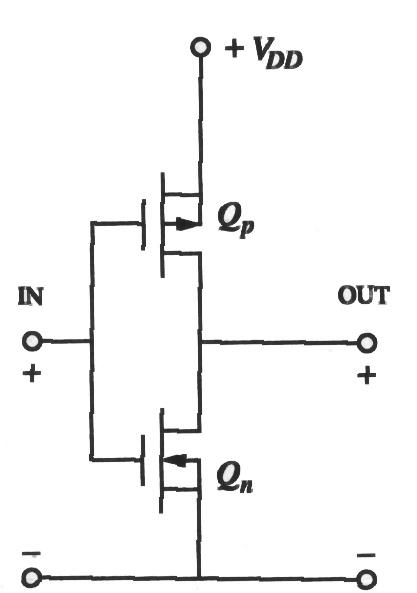
\includegraphics[width=0.5\linewidth]{fig/11-CMOS_NAND_schema}\\
Alacsony logikai bemeneti fesztültségnél az N-csatornás Q\textsubscript{n} tranzisztor lezárt állapotban van és a P-csatornás Q\textsubscript{p} tranzisztor nyitott állapotban így a kimenet logikai magas szinten lesz (megközelítőleg V\textsubscript{DD} értékű). Ha a bemenetre logikai magas szint kerül, akkor Q\textsubscript{n} tranzisztor kinyit és Q\textsubscript{p} tranzisztor lezár, ezáltal logikai alacsony szint kerül a kimenetre. Ha a működési frekvencia megnövekszik, vele együtt nő a teljesítményfelvétel is a tranzisztorok kapcsolási ideje miatt kialakuló tápáramfogyasztás miatt. 

A C-MOS áramkörök tápfeszültsége +3 és +15 V közötti értéket vehet fel. Egy nem-és kapu terjedési késleltetési ideje átlagosan 25 ns, a nyugalmi teljesítmény: 50 nW

A C-MOS áramkörök nagy jelentőségű változata az SOS (Silicon on Sapphire). Szilícium helyett zafír hordozóra alakítják a a C-MOS-okat. Az áramköri elemek között a szigetelési ellenállás nagyon nagy értékű,ezáltal csökken a hordozók kapacitása és nagyságrendekkel nő a sebesség is (1-2 ns). Jelentősen csökken az áramkör nyugalmi teljesítménye is.

\subsection{Különböző áramköri családok csatlakoztatása.}
A logikai függvények fizikai megvalósításához a gyártó cégek bizonyos alapáramkör választékot (családokat) alakítanak ki. Az áramkörök összekapcsolását a katalógusokban található jellemző adataik közlése és egyeztetése teszi lehetővé. A digitális technikában a pozitív logika terjedt el, és az áramkörök pozitív feszültségrendszerben dolgoznak. Amikor
csatlakoztatjuk a különböző áramkörcsaládokat, a következő jellemzőket kell megvizsgálni:
\begin{enumdescript}
	\item[Tápfeszültség] az áramkör működéséhez szükséges feszültség
	\item[Logikai szintek] U\textsubscript{Hmin} és U\textsubscript{Hmax} valamint U\textsubscript{Lmin} és U\textsubscript{Lmax} jellemző értékek
	\item[Zajtartalék, zajérzékenység] feszültségingadozás, ami még nem változtatja meg az állapotot
	\item[Bementeti terhelhetőség] egységterhelés, mind alacsony mind magas logikai szinten
	\item[Kimenteti terhelhetőség] károsodás nélkül a kimenetet képes hajtani
	\item[Teljesítményfelvétel] teljesítményigény 50\%-os terhelésnél
	\item[Jelkésleltetési idő] a kimenet reagál a bemenet hatására, amihez idő kell
\end{enumdescript}

\subsection{Kombinációs és szekvenciális hálózatok. A/D és D/A átalakítók.}
\paragraph{Kombinációs hálózatok} \emph{időfüggetlen} logikai függvényeket valósítanak meg, memória nélküli logikai áramkörök, a kimeneti logikai változókat az adott időpontban megjelenő bemeneti logikai változók határozzák meg, az áramköröket IC-kel (Integrated circuit) valósítják meg, a logikai alapfüggvényeket megvalósító áramköröket logikai kapuknak nevezzük, egy IC-n belül több logikai kapu is található.

\paragraph{Szekvenciális (sorrendi) hálózatok} \emph{időfüggő} logikai függvényeket valósítanak meg, a kimeneti események alakulását a pillanatnyi bemeneti feltételek mellett a korábbi időpillanatokban bekövetkezett kimeneti események is befolyásolják, attól függően, hogy az állapotváltozás hogyan következik be két csoportot különbözetünk meg:
\begin{description}
	\item[Aszinkron] a kimenet előző állapotától való függést visszacsatolással vagy tárolókkal valósítják meg, a kimenet a bemenetre azonnal reagál
	\item[Szinkron] az állapotváltozás a kimeneten egy engedélyező jel (Clock) hatására, azzal azonos fázisban zajlik le, a kimenet előző állapotától való függést tárolókkal oldják meg.
\end{description}

Kombinációs és szekvenciális hálózatok típusai:
\begin{itemize}[nosep]
	\item R-S tároló
	\item Inverz R-S tároló
	\item J-K tároló
	\item T tároló
	\item D tároló
\end{itemize}

\paragraph{A/D átalakítók}
Feladatuk, hogy a bemenetre érkező „A” analóg jelnek megfelelő „D” digitális jelet (bináris számot) állítson elő a kimeneten, a működéshez szükséges egy R referencia (ált. egy U R referenciafeszültség), melyhez a konverter az A analóg mennyiségét viszonyítja és amely a kimeneti feszültség maximális értékét is meghatározza. Az A/D átalakító kvantál (viszonyítási tartományt használ) a digitális jelek előállításához. A digitalizáláshoz elemi lépcsőket kell használni, és minden lépcsőhöz egy digitális mennyiséget (bináris szám) kell rendelni. Az analóg jel annál pontosabban ábrázolható minél kisebb egy elemi lépcső, vagy kvantum nagysága. Az A/D átalakítóknak annál nagyobb a felbontóképessége minél több bit áll rendelkezésre az ábrázoláshoz. Az átalakítók felbontásának növelése az áramköri megvalósítást nehezíti, drágítja. A kis pontosság-igény esetén elég a 8 bit-es (256 elemi lépcső), nagyobb pontosságot biztosítanak a 10,12,14 bites átalakítók és nagy pontosságú rendszerekben 16,18,20 biteseket alkalmaznak.

\paragraph{D/A átalakítók}
Feladatuk, hogy a bemenetre érkező „D” digitális jelnek megfelelő „A” analóg jelet (általában feszültséget vagy áramot) állítson elő a kimeneten, működéséhez szükséges egy U\textsubscript{R} referenciafeszültség (nagyon pontos feszültségforrás), amelyből a kimeneti feszültséget származtatjuk és ez határozza meg a kimeneti feszültség maximális értékét (végkitérését) is. A digitális technikában többnyire bináris alakban állnak rendelkezésre, valamilyen meghatározott kódban kifejezve, ezt a kódot a D/A átalakítónak ismerni kell, csak ezeket a meghatározott bináris kódokat tudják analóg jellé alakítani. Az ideális D/A átalakítók kimeneti jele egyenesen arányos a bemenetükre digitálisan adott szám értékével. A pontosságot itt is az elemi lépcsők száma határozza meg, minél kisebb egy ilyen lépcső, annál pontosabb az átalakítás. Vannak soros és párhuzamos működésű átalakítók és megkülönböztetünk közvetlen és közvetett elvű átalakítókat.